\chapter{Арифметические операции. Сложение}

\section{Как складывать двоичные числа}

Логическое сложение мы уже видели. Там $1+1=1$, это не подходит для того,
чтобы делать обычные арифметические вычисления. Ведь мы хотим получить
$1_2+1_2=10_2$.

Посмотрим, как складывать два числа, например $14$ и $7$.
Для этого переведём их в двоичную систему счисления (всё равно ведь компьютеры работают в ней)
и запишем их для сложения в столбик:

$$
\begin{array}{ccccc}
  & 1 & 1 & 1 & 0 \\
+ & 0 & 1 & 1 & 1 \\ \hline
  & ? & ? & ? & ? \\
\end{array}
$$

Сложение в столбик как обычно делается справа налево. Только здесь ещё нужно помнить,
что мы работаем в двоичной, а не в десятичной системе счисления.
Справа складываются $0$ и $1$, очевидно, что получается $1$:

$$
\begin{array}{ccccc}
  & 1 & 1 & 1 & 0 \\
+ & 0 & 1 & 1 & 1 \\ \hline
  & ? & ? & ? & 1 \\
\end{array}
$$

Следующая пара цифр это $1$ и $1$. Мы уже знаем, что должно получиться~$10$.
А это значит, что в текущем разряде остаётся~$0$, а лишняя единица должна перейти
в следующий разряд:

$$
\begin{array}{ccccc}
  & 1 & 1 & 1 & 0 \\
+ & 0 & 1 & 1 & 1 \\ \hline
  & ? & ?+1 & 0 & 1 \\
\end{array}
$$

Дальше мы снова складываем $1$ и $1$, но к ним ещё добавляется перенос из предыдущего разряда.
То есть будет $1+1+1=11$. Значит в текущем разряде результата теперь единица,
а в следующий снова идёт бит переноса.

$$
\begin{array}{ccccc}
  & 1 & 1 & 1 & 0 \\
+ & 0 & 1 & 1 & 1 \\ \hline
  & ?+1 & 1 & 0 & 1 \\
\end{array}
$$

Последняя сумма уже знакома: $1+0+1=10$. То есть в текущий разряд результата записывается~$0$,
а в следующий идёт~$1$.

$$
\begin{array}{ccccc}
  & 1 & 1 & 1 & 0 \\
+ & 0 & 1 & 1 & 1 \\ \hline
1 & 0 & 1 & 0 & 1 \\
\end{array}
$$

Если перевести $10101_2$ в десятичную систему, то получится $16+4+1=21$, как и ожидалось.
Теперь нужно придумать, как такую сумму считать с помощью реле.

\section{Сумматор}

Схему сложения удобнее всего строить из однотипных компонентов, складывающих
пару битов.
Сумма двух битов может дать результат $0_2$, $1_2$ или $10_2$.
То есть при сложении получается уже двухбитовое число: младший бит суммы
и старший бит суммы, который называется битом переноса, или битом переполнения, или carry, или $CY$.

Для сложения чисел из нескольких битов, нужно соединить однобитные сумматоры в цепочку
и передавать биты переноса от предыдущего сумматора к следующему.

Таким образом, однобитный сумматор получает на вход бит переноса и два бита-слагаемых, а на выходе
у него тоже бит переноса и однобитная сумма. С помощью набора таких сумматоров можно
сложить числа любой длины.

% TODO: логическое выражение для сумматора

Особенность реализации сумматора с помощью реле в том, что на входе
требуется не только перенос ($CY$), но и инвертированный перенос ($\textasciitilde CY$).
Такой же инвертированный перенос можно генерировать и на выходе.

\begin{center}
\includegraphics{schemes/add.png}
\end{center}

Эту схему сумматора изобрёл Конрад Цузе для своих компьютеров в 1940х годах.
Несколько таких сумматоров можно соединить последовательно, чтобы
складывать многобитные числа. Для этого соединяются соответствующие входы
и выходы для переноса и инвертированного переноса, чтобы
переполнение переходило из бита~$0$ в бит~$1$, из бита~$1$ в бит~$2$ и
так далее.

\section{Модуль сумматора}

%
\includegraphics[width=\columnwidth]{schemes_components/adder.png}

\begin{center}
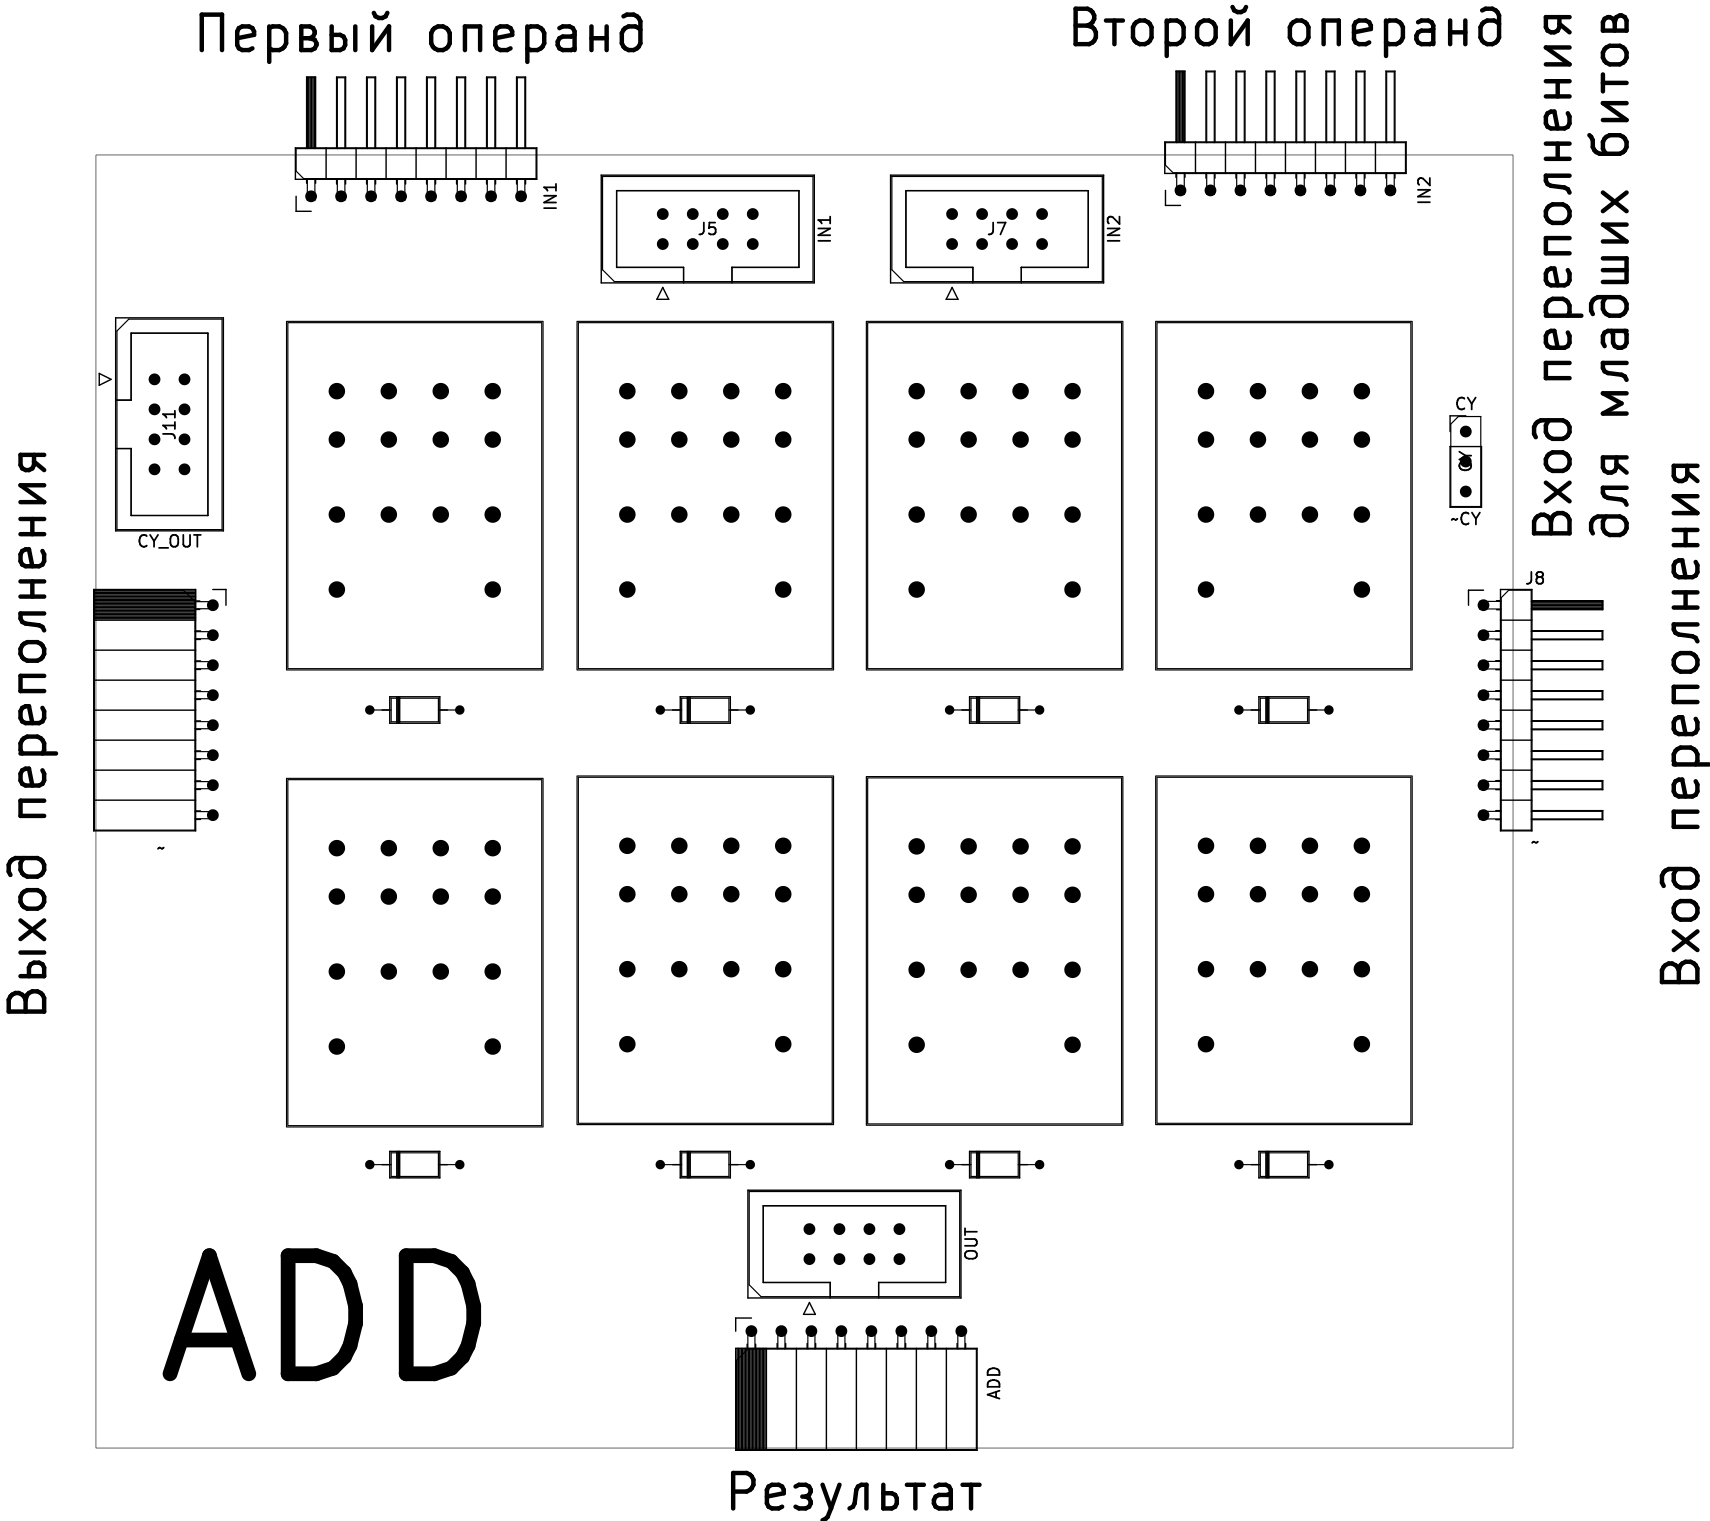
\includegraphics{boards/adder.png}
\end{center}

Сумматор складывает два четырёхбитных числа, один бит переноса и выдаёт четырёхбитное число и бит переноса.

Модуль имеет следующие разъёмы:
\begin{itemize}
  \item Слева и справа: шины для каскадирования нескольких модулей.
        Справа к сумматору приходит сигнал переноса от сумматора младших битов (если он подключен),
        а помощью шины слева получившийся в результате сложения перенос можно
        передать на следующий сумматор, записать в регистр или использовать
        в других логических схемах.
  \item Рядом с правым разъёмом есть перемычка для включения или выключения
        бита переноса, если каскадирование не используется.
        В этом случае перемычка обязательно должна быть в одном из двух положений.
        Если же справа подключен другой сумматор, то перемычку нужно убрать.
        Без перемычки (или без замены её тумблерами) не получится, потому что один
        из двух сигналов (перенос или инвертированный перенос) должен быть единицей.
  \item Сверху: разъёмы для подключения сигналов-операндов.
        Можно подсоединить к шинам, а можно к модулям переключателей или регистрам.
  \item Снизу: разъём, откуда можно считать сумму операндов.
\end{itemize}

% \subsection{Подготовка}

% \begin{enumerate}
%     \item Придумайте, как можно было бы составить схему из реле, чтобы вычислять сумму однобитовых чисел.
%     \item Как можно использовать предыдущую схему для вычисления суммы двухбитовых чисел?
% \end{enumerate}

\section{Практикум}

\subsection{Работа модуля}

Список модулей:
\begin{itemize}
    \item Модуль переключателей: $3$ штуки
    \item Сумматор: $1$ штука
    \item Регистровый модуль: $1$ штука
\end{itemize}

Ко входам модуля подключаются два модуля с тумблерами, а к выходам --- регистр,
куда будет записываться результат.

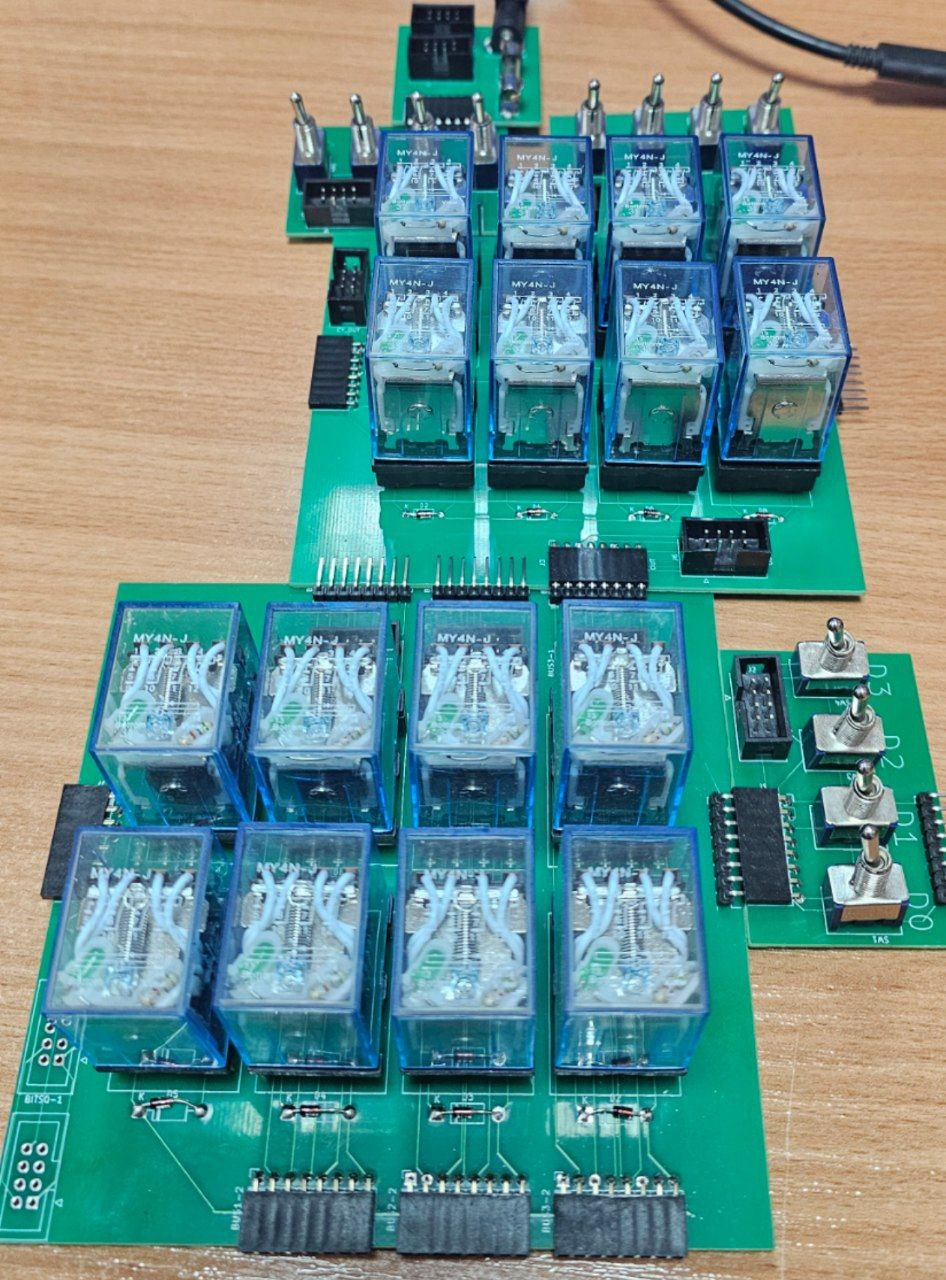
\includegraphics[width=0.5\columnwidth]{photo/adder.jpg}

\begin{enumerate}
    \item Отключите все управляющие сигналы.
    \item Установите перемычку для подачи сигнала на $\textasciitilde CY$.
    \item Наберите на тумблерах первого операнда значение $0011$ (число $3$).
    \item Наберите на тумблерах второго операнда значение $1010$ (число $10$).
    \item Подключите выходной регистр к шине $3$. Убедитесь, что в него записалось значение $1101$ (число $13$).
    \item Отключите регистр от шины, сбросьте его значение.
    \item Установите перемычку для подачи сигнала на $CY$.
    \item Подключите выходной регистр к шине $3$. Убедитесь, что в него записалось значение $1110$ (число $14$).
\end{enumerate}


\section{Задачи}

\begin{enumerate}
    \item Соберите устройство для сложения значения из регистра с константой, набранной на тумблерах.
          Должна быть предусмотрена запись результата обратно в регистр.
          Дальше управляйте сигналами таким образом, чтобы к регистру последовательно
          прибавлялась единица, пока он не достигнет значения $1111$.
          Тут необходимо использовать два регистровых модуля: из одного будет считываться операнд для сложения,
          а во второй записываться результат.
\end{enumerate}

\subsection{Восьмибитный сумматор}

Модули сумматоров можно объединять, как и регистры, чтобы работать с данными большей разрядности.
Для этого используются боковые разъёмы, через которые
передаются сигналы переноса.

\subsection{Практикум}

% TODO: запись восьмибитного значения в регистр

Соедините два регистра и два сумматора. Шина $3$ регистров подключается к сумматору.
У правого (младшего) сумматора входящий перенос перемычкой устанавливается в $0$.
У левого (старшего) сумматора перемычка для переноса убирается, потому что
сигнал переноса приходит от младших битов (из правого сумматора).

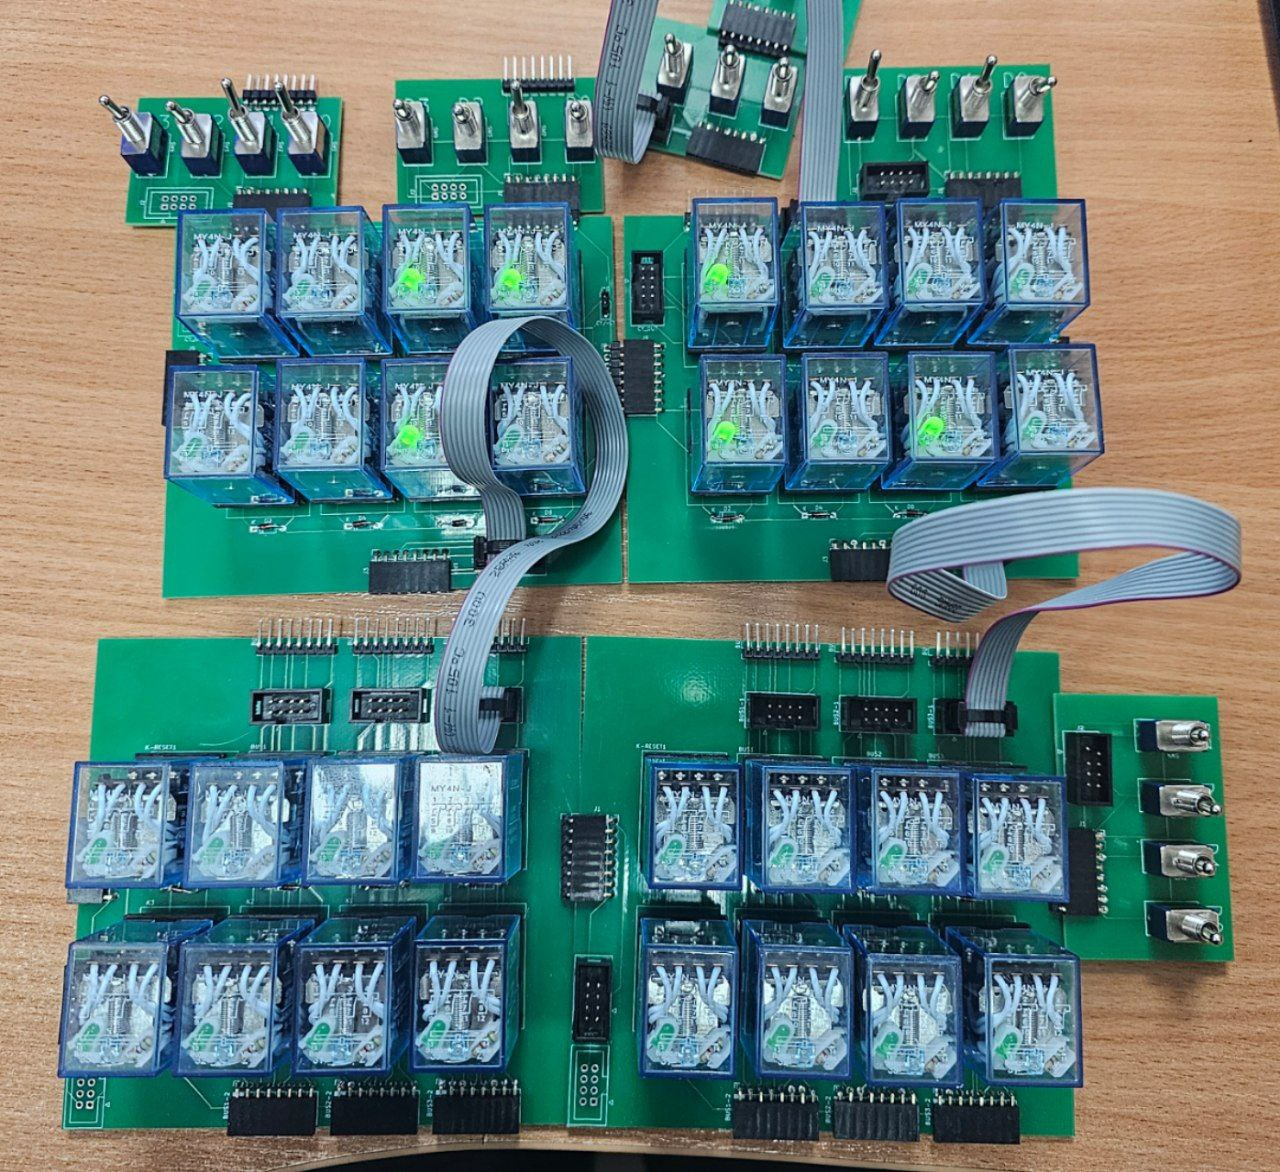
\includegraphics[width=0.5\columnwidth]{photo/8bit.jpg}

\begin{enumerate}
    \item Отключите все управляющие сигналы.
    \item Наберите входные данные $0011 1001$ и $0010 1001$.
    \item Подключите выход сумматора к регистру тумблером $D3$.
    \item Проверьте, что в результате получилось число $0110 0010$.
\end{enumerate}

